% -----------------------------------------------------------------------------
% Centre for Industrial Software - SDU
% Semester Project 3 - 2026 Report Template
% -----------------------------------------------------------------------------

\documentclass[12pt, a4paper, openany]{report}

% -----------------------------------------------------------------------------
% PACKAGES
% -----------------------------------------------------------------------------
\usepackage{microtype}                                        % Aesthetic typography spacing
\usepackage{cmbright}                                         % Clean sans-serif font
\usepackage[utf8]{inputenc}                                   % UTF-8 support
\usepackage[T1]{fontenc}                                      % Font encoding
\usepackage[colorlinks=true, allcolors=black]{hyperref}       % Hyperlinks
\usepackage{fancyhdr}                                         % Headers and footers
\usepackage{amsmath,amssymb}                                  % Math packages
\usepackage{graphicx}                                         % Graphics
\usepackage{booktabs}                                         % Professional tables
\usepackage[english]{babel}                                   % Language
\usepackage[a4paper,
            top=35mm,
            bottom=30mm,
            left=35mm,
            right=25mm]{geometry}                             % Page margins
\usepackage{csquotes}                                         % Context-sensitive quotation
\usepackage{lipsum}                                           % Lorem ipsum generator
\usepackage{xcolor}                                           % Color support
\usepackage{caption}                                          % Captions
\usepackage{cite}                                             % IEEE style citation handling
\usepackage{listings}                                         % Source code listings
\usepackage{titlesec}                                         % Title formatting
\usepackage{float}                                            % Floating environments
\usepackage{enumitem}                                         % Customizable lists
\usepackage{parskip}                                          % Space between paragraphs instead of indent
\usepackage{tikz}                                             % TikZ diagrams and placeholder graphics

% -----------------------------------------------------------------------------
% USER VARIABLES & DEFINITIONS
% -----------------------------------------------------------------------------
\newcommand{\theInstitute}{Centre for Industrial Software}
\newcommand{\theSemester}{Semester Project 3 -- 2026}
\newcommand{\theTitle}{uniDesk}
\newcommand{\theSubtitle}{Group 12 -- LINAK Desk Usage Supervision}
\newcommand{\theSupervisor}{[Supervisor Name]}
\newcommand{\theGroup}{Group 12}

\definecolor{mygrey}{RGB}{64,64,64}
\definecolor{sdublue}{RGB}{0,51,102}

% Header and Footer configuration
\pagestyle{fancy}
\fancyhf{}
\fancyhead[L]{\small\textit{\theTitle}}
\fancyhead[R]{\small\textit{\nouppercase{\leftmark}}}
\fancyfoot[C]{\thepage}
\setlength{\headheight}{16pt}
\renewcommand{\headrulewidth}{0.4pt}
\renewcommand{\footrulewidth}{0pt}

% Plain page style (used for chapter opening pages)
\fancypagestyle{plain}{
  \fancyhf{}
  \fancyhead[L]{\small\textit{\theTitle}}
  \fancyfoot[C]{\thepage}
  \renewcommand{\headrulewidth}{0.4pt}
}

% -----------------------------------------------------------------------------
% DOCUMENT
% -----------------------------------------------------------------------------
\begin{document}

% -----------------------------------------------------------------------------
% PAGE 1: TITLE PAGE / COVER
% -----------------------------------------------------------------------------
\begin{titlepage}
\pagestyle{empty}

\noindent
{\textbf{sdu.dk} \hfill \textbf{\#sdudk}}\\[0.5cm]
\noindent
{\large \textsc{\theInstitute}}\\[0.2cm]
\noindent
{\large \theSemester}

\vspace{3.5cm}

\begin{center}
\hrule\vspace{0.8cm}
{\huge \textbf{\textcolor{mygrey}{\theTitle}}}\\[0.4cm]
{\Large \textit{\theSubtitle}}
\vspace{0.8cm}\hrule
\end{center}

\vspace{2.2cm}

\begin{center}
{\large \textbf{Project Participants:}}\\[0.4cm]
\begin{tabular}{ll}
Filip Cunderlik & ficun25@student.sdu.dk \\
Dominik Bezo & dobez25@student.sdu.dk \\
Daniel Falat & dafal25@student.sdu.dk \\
Pavel Seliavko & pasel25@student.sdu.dk \\
Zoe Elea Schiwy & zosch25@student.sdu.dk \\
David Nicolae Petrescu & davpe25@student.sdu.dk \\
\end{tabular}

\vspace{1.2cm}

{\large \textbf{Supervisor:}}\\[0.2cm]
{\large \theSupervisor}

\vfill
{\small \today}
\end{center}

\end{titlepage}

% -----------------------------------------------------------------------------
% FRONT MATTER
% -----------------------------------------------------------------------------
\pagenumbering{roman}
\setcounter{page}{2}

% PAGE 2: GROUP MEMBER CONTRIBUTIONS & DEVICE HISTORY
\chapter*{Group Contributions and Device History}

\section*{Group Members Contributions}
\noindent All group members contributed equally to the project unless specified otherwise below:
\begin{itemize}
    \item Filip Cunderlik: Equal contribution (or [X]\%)
    \item Dominik Bezo: Equal contribution (or [X]\%)
    \item Daniel Falat: Equal contribution (or [X]\%)
    \item Pavel Seliavko: Equal contribution (or [X]\%)
    \item Zoe Elea Schiwy: Equal contribution (or [X]\%)
    \item David Nicolae Petrescu: Equal contribution (or [X]\%)
\end{itemize}

\vspace{1.5cm}

\section*{Device History}
\noindent [Short history of the Device in your name, max. \textonehalf\ page. Building off the LINAK Desk Usage Supervision case study and the uniDesk system.]

\newpage

% PAGE 3: ABSTRACT
\chapter*{Abstract}

[The Abstract of a technical report is a concise summary that provides an overview of the entire report. It typically includes the following key elements:
\begin{itemize}
    \item \textbf{Purpose of the Project}
    \begin{itemize}
        \item State the problem the project addresses.
        \item Mention the motivation or context for undertaking the work.
    \end{itemize}
    \item \textbf{Objectives}
    \begin{itemize}
        \item Briefly describe the main goals of the project.
    \end{itemize}
    \item \textbf{Methods or Approach}
    \begin{itemize}
        \item Highlight the methodology or techniques used to solve the problem.
        \item Mention any tools, technologies, or frameworks employed.
    \end{itemize}
    \item \textbf{Key Results or Findings}
    \begin{itemize}
        \item Summarize the most important outcomes or achievements of the project.
        \item Mention whether the goals were met and what was accomplished.
    \end{itemize}
    \item \textbf{Conclusion}
    \begin{itemize}
        \item Provide a high-level reflection on the impact or significance of the work.
        \item Optionally, hint at future possibilities or improvements.
    \end{itemize}
\end{itemize}

The Abstract should be:
\begin{itemize}
    \item \textbf{Brief:} Typically, 150--250 words.
    \item \textbf{Self-contained:} Readers should understand the project without reading the rest of the report.
    \item \textbf{Informative:} Focus on what was done, how, and the results.
    \item \textbf{Non-technical:} Avoid excessive jargon or technical details; it should be understandable by a broader audience.
\end{itemize}

It should be written last, after completing the report, to accurately reflect its content.]

\newpage

% PAGE 4: DECLARATION OF GENAI USAGE
\chapter*{Declaration of GenAI Usage}

[The use of generative artificial intelligence (GenAI) must be declared in accordance with SDU regulations and guidance. Students are responsible for their use of AI-generated output, and the intellectual work presented in the report must remain their own. The declaration should make it clear to the reader how generative AI contributed to the final work.

If generative AI tools were used during the project, briefly describe:
\begin{itemize}
    \item Tools used, e.g. Microsoft Copilot, ChatGPT, GitHub Copilot, or other AI-based tools
    \item Purpose and extent of use, e.g. brainstorming, structuring the report, literature search, language improvement, summarization, analysis, generation or modification of text, programming, or generation of other material
    \item Where relevant, indicate the use of generative AI at the appropriate place in the report, source code, or other project material
\end{itemize}

If generative AI was not used, state this explicitly.

Students must follow the current SDU rules and guidance concerning generative AI. Consult:
\begin{itemize}
    \item SDU Library: SDU regulations and guidance on generative AI
    \item Software Engineering S\o{}nderborg: Guide to the use of generative AI
\end{itemize}

The Software Engineering guidance provides more detailed instructions for different forms of AI use. For example, AI-generated or AI-paraphrased text requires appropriate declaration/citation, while uses such as report structuring, brainstorming, language assistance, analysis, and programming should be described at a relevant point in the assignment.]

\newpage

% PAGE 5: TABLE OF CONTENTS
\tableofcontents
\newpage

% PAGE 6: LIST OF TABLES
\listoftables
\newpage

% PAGE 7: LIST OF FIGURES
\listoffigures
\newpage

% -----------------------------------------------------------------------------
% MAIN CONTENT CHAPTERS
% -----------------------------------------------------------------------------
\pagenumbering{arabic}
\setcounter{page}{8}

% CHAPTER 1: INTRODUCTION
\chapter{Introduction}
\label{chap:introduction}

[Provides an overview of the project, including the context, objectives, scope, and importance. This includes the desk use case as well the 3rd semester structure. It explains the problem being addressed and sets the stage for the subsequent chapters.]

\section{Motivation}
\label{sec:motivation}
[Lorem ipsum]

\section{Objective}
\label{sec:objective}
[Lorem ipsum]

\section{Delimitation}
\label{sec:delimitation}
[After introducing the project and its objectives, include a paragraph explaining:
\begin{itemize}
    \item What the project will not address (e.g., specific features, areas, or use cases that are out of scope)
    \item Constraints or limitations (e.g., time, budget, technology, or resources)
\end{itemize}]



% CHAPTER 2: METHODOLOGY
\chapter{Methodology}
\label{chap:methodology}

[Describes the approach and techniques employed to address the problem. This could include research methods, tools, technologies, and frameworks used during the project and the 3rd semester courses.

You build the project based on the experience and knowledge accumulated during the previous semesters---don't forget that.]

\begin{figure}[htbp]
    \centering
    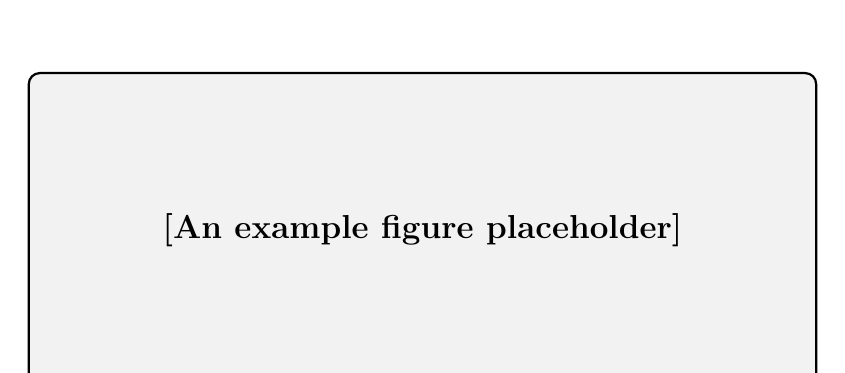
\begin{tikzpicture}
        \draw[thick, fill=gray!10, rounded corners=4pt] (0,0) rectangle (10, 4);
        \node at (5, 2) {\large \textbf{[An example figure placeholder]}};
    \end{tikzpicture}
    \caption{An example figure}
    \label{fig:example_figure}
\end{figure}

\section{[Sub-section]}
\label{sec:methodology_subsection}
[Lorem ipsum]

\subsection{[Sub-sub-section]}
\label{subsec:methodology_subsubsection}
[Lorem ipsum]



% CHAPTER 3: PROBLEM ANALYSIS
\chapter{Problem Analysis}
\label{chap:problem_analysis}

[A detailed breakdown of the problem being tackled. This section analyses the key challenges, potential bottlenecks, and constraints. It may also include a review of related work or literature.]

\section{[Sub-section]}
\label{sec:problem_analysis_subsection}
[Lorem ipsum]

\subsection{[Sub-sub-section]}
\label{subsec:problem_analysis_subsubsection}
[Lorem ipsum]



% CHAPTER 4: REQUIREMENTS
\chapter{Requirements}
\label{chap:requirements}

[Lists the functional and non-functional requirements for the project, clearly stating what the system, application, or solution is expected to achieve.]

\begin{table}[htbp]
\centering
\caption{An example table}
\label{tab:example_table}
\begin{tabular}{ccc}
\toprule
\textbf{Feature / ID} & \textbf{Description} & \textbf{Status} \\
\midrule
X & X & X \\
X & X & X \\
X & X & X \\
\bottomrule
\end{tabular}
\end{table}

\section{[Sub-section]}
\label{sec:requirements_subsection}
[Lorem ipsum]

\subsection{[Sub-sub-section]}
\label{subsec:requirements_subsubsection}
[Lorem ipsum]



% CHAPTER 5: DESIGN
\chapter{Design}
\label{chap:design}

[Outlines the architecture, system design, and key components of the project. This chapter may include diagrams like UML models, flowcharts, or block diagrams to visually represent the design.]

\section{[Sub-section]}
\label{sec:design_subsection}
[Lorem ipsum]

\subsection{[Sub-sub-section]}
\label{subsec:design_subsubsection}
[Lorem ipsum]



% CHAPTER 6: IMPLEMENTATION
\chapter{Implementation}
\label{chap:implementation}

[Documents the process of developing the solution, including key algorithms, code snippets, libraries, and tools used. Focus is on the technical realization of the design.]

\section{[Sub-section]}
\label{sec:implementation_subsection}
[Lorem ipsum]

\subsection{[Sub-sub-section]}
\label{subsec:implementation_subsubsection}
[Lorem ipsum]



% CHAPTER 7: VALIDATION
\chapter{Validation}
\label{chap:validation}

[Details the testing and validation processes to ensure the system meets the specified requirements. Includes test cases, results, and analysis of the performance or functionality of the solution.]

\section{[Sub-section]}
\label{sec:validation_subsection}
[Lorem ipsum]

\subsection{[Sub-sub-section]}
\label{subsec:validation_subsubsection}
[Lorem ipsum]



% CHAPTER 8: CONCLUSION
\chapter{Conclusion}
\label{chap:conclusion}

[Summarizes the outcomes of the project, lessons learned, and areas for future improvement or further study. It may also reflect on how well the objectives were achieved.]

\section{Summary}
\label{sec:summary}
[Lorem ipsum]

\section{Future Work}
\label{sec:future_work}
[Lorem ipsum]



% -----------------------------------------------------------------------------
% REFERENCES (IEEE Style)
% -----------------------------------------------------------------------------
\clearpage
\phantomsection
\nocite{*} % Shows the IEEE references
\addcontentsline{toc}{chapter}{References}
\bibliographystyle{IEEEtran}
\bibliography{References}

% -----------------------------------------------------------------------------
% APPENDIX
% -----------------------------------------------------------------------------
\clearpage
\phantomsection
\addcontentsline{toc}{chapter}{Appendix A}
\chapter*{Appendix A}
\label{chap:appendix_a}

[The Appendix sections in the report is used to include supplementary information that is too detailed or extensive to be included in the main chapters but is still important for understanding the project.

Common appendices:
\begin{itemize}
    \item Raw data or detailed calculations
    \item Code snippets or algorithms
    \item Detailed figures, graphs, or tables
    \item Technical specifications
    \item Test cases and results
    \item Meeting minutes or project logs
    \item User manuals or guides
    \item Legal documentation, agreements
\end{itemize}]


\end{document}
